\section{Plano da atenção primária e equipes móveis}

O plano mantém as 22 UBS existentes e abre nove novas, três urbanas e seis rurais, identificadas como N1
a N9. A rede passa a ter 39 eSF e 192 ACS fixos. As UBS existentes mantêm as suas 23 eSF e 140 ACS e
ganham apenas um ACS, na UBS Morada Nova, porque o número de salas não comporta novas equipes. As três
UBS urbanas novas concentram 10 das 16 eSF adicionais, e cada UBS rural tem uma equipe. Duas equipes
móveis, com quatro ACS, completam a rede a partir da UBS Alto do Rosário.

A Tabela~\ref{tab:cobertura} compara as duas medidas de cobertura, e a Figura~\ref{fig:mapa} mostra a
rede antes e depois do plano. A cobertura geográfica passa de 93,4\% para 97,7\%, e a cobertura com
capacidade, de 65,6\% para 97,7\%. Os 2.385 habitantes que continuam a mais de 3 km de uma UBS, em sete
setores rurais, são atendidos pelas equipes móveis (Tabela~\ref{tab:movel}), o que leva a cobertura
potencial a 100\% da população.

\begin{table}[htbp]\centering
\caption{Cobertura potencial da população projetada para 2026}\label{tab:cobertura}
\begin{tabular}{lrr}\toprule
Rede & Geográfica, 3 km (\%) & Com capacidade (\%)\\\midrule
Rede atual (22 UBS) & 93,40 & 65,62\\
Rede proposta (31 UBS) & 97,71 & 97,71\\
Rede proposta com equipes móveis & & 100,00\\
\bottomrule\end{tabular}
\fonte{Resultados do modelo, com dados de \citet{ibge2026est} e \citet{cnes2026}.}
\nota{A cobertura com capacidade limita a carga de cada UBS a 3.000 habitantes por eSF e 750 por ACS.
A cobertura móvel é potencial e depende das hipóteses de alcance e capacidade da Seção~\ref{sec:movel}.}
\end{table}

\begin{figure}[p]\centering
\begin{subfigure}{\linewidth}\centering
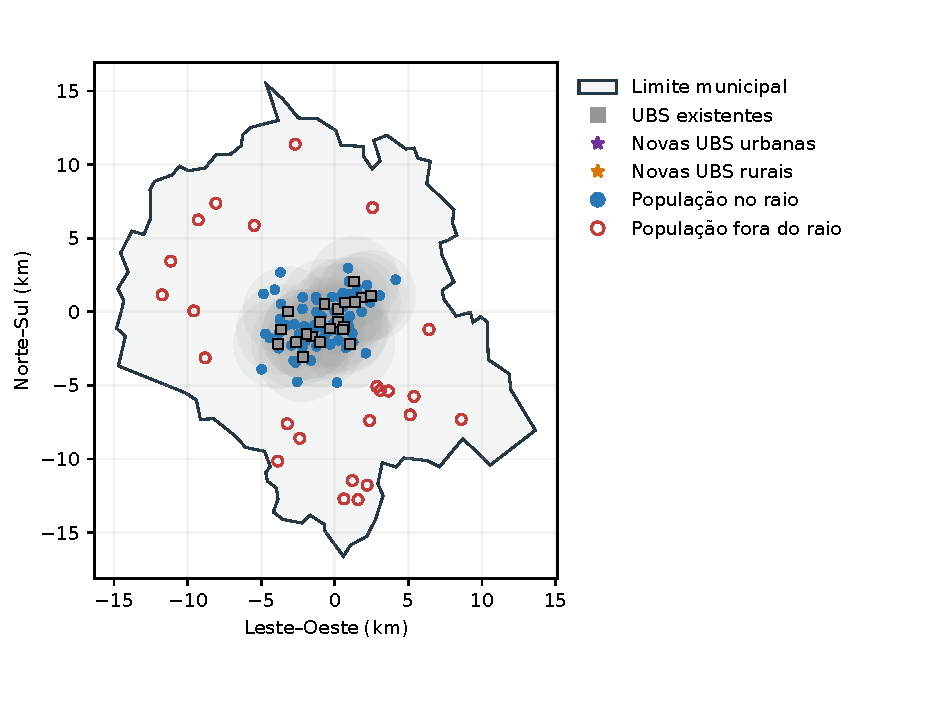
\includegraphics[width=.92\linewidth,height=.38\textheight,keepaspectratio]{figuras/mapa_rede_atual.pdf}
\caption{Rede atual com 22 UBS}\label{fig:mapa_atual}
\end{subfigure}

\vspace{10pt}
\begin{subfigure}{\linewidth}\centering
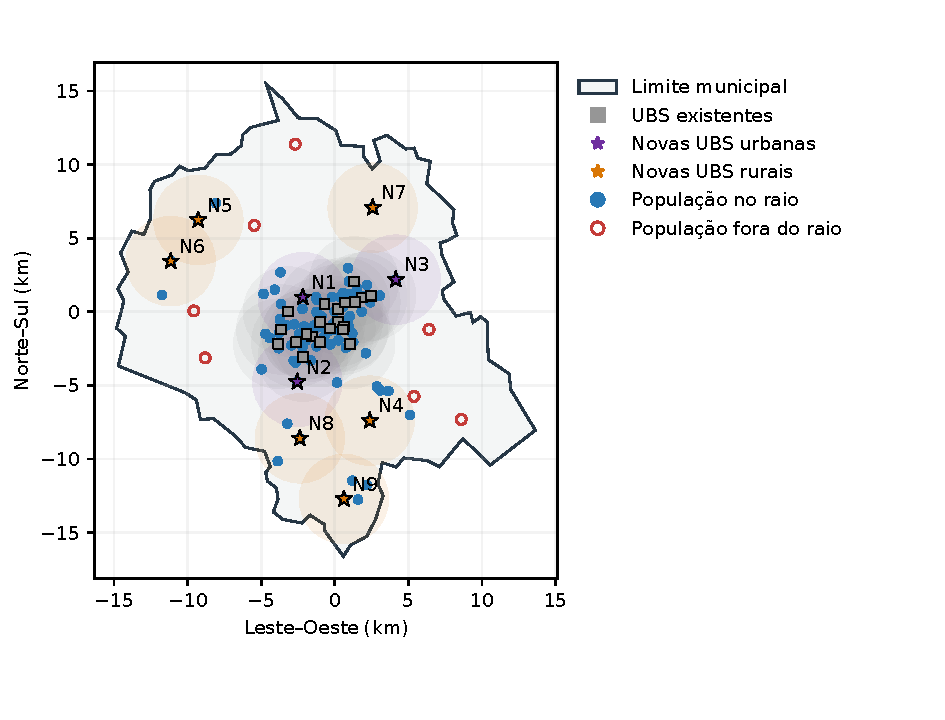
\includegraphics[width=.92\linewidth,height=.38\textheight,keepaspectratio]{figuras/mapa_plano_par.pdf}
\caption{Plano proposto com as 22 UBS existentes e as novas UBS N1 a N9}\label{fig:mapa_plano}
\end{subfigure}
\caption{Localização das UBS e cobertura geográfica no raio de 3 km, antes e depois do plano}\label{fig:mapa}
\fonte{Resultados do modelo, com dados de \citet{ibge2022} e \citet{cnes2026}.}
\nota{Códigos N1 a N9 conforme a Tabela~\ref{tab:unidades}. A base das equipes móveis (UBS Alto do Rosário)
não é representada.}
\end{figure}

A Figura~\ref{fig:acesso} mostra a população acumulada segundo a distância até a UBS mais próxima. Na
rede atual, os setores rurais mais afastados chegam a 10,4 km de uma UBS, e com as novas unidades a maior
distância cai para 7,0 km. Essa curva mede apenas a proximidade, sem levar em conta a capacidade das
equipes, que é o foco da comparação seguinte. A população que mora a mais de 3 km de uma UBS cai de
6.862 para 2.385 habitantes.

\begin{figure}[htbp]\centering
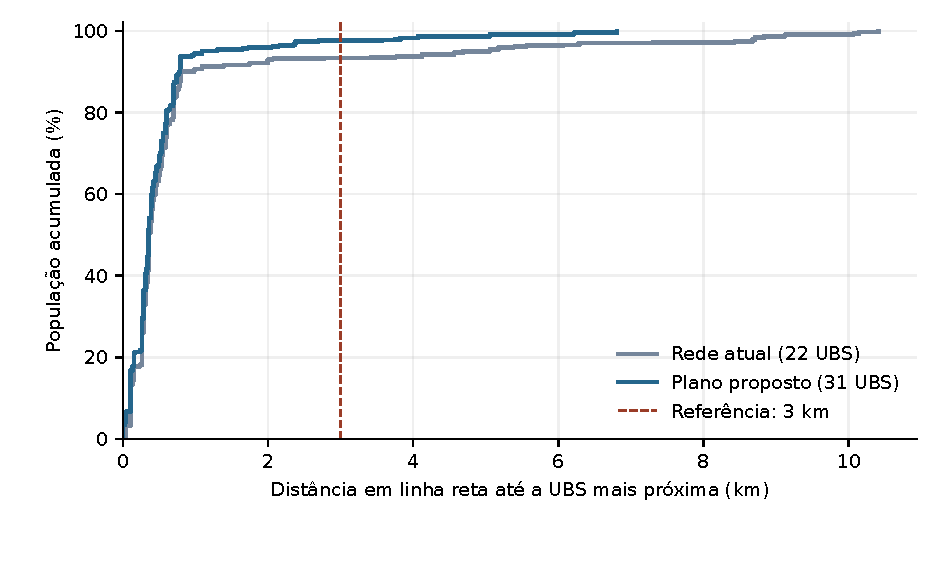
\includegraphics[width=.85\linewidth]{figuras/curva_acesso_geografico.pdf}
\caption{População acumulada segundo a distância até a UBS mais próxima, na rede atual e no plano proposto}\label{fig:acesso}
\fonte{Resultados do modelo de localização e dimensionamento.}
\end{figure}

O modelo nunca aloca a uma UBS mais pessoas do que as suas equipes comportam, e por isso a cobertura com
capacidade mede quantas pessoas podem de fato ser acompanhadas por uma equipe. Na rede atual, as 23 eSF
comportam 69.000 habitantes para uma população de 104.002. Com o limite dos ACS, a capacidade efetiva cai
para 68.250, e 35.752 pessoas ficam sem equipe disponível, o que explica a cobertura com capacidade de
65,6\%.

No plano, as 39 eSF comportam 117.000 habitantes. As UBS existentes continuam lotadas, e a expansão vem
das novas unidades. As urbanas atendem 28.560 habitantes, 95\% da capacidade das suas equipes, e as rurais
atendem 6.443, cerca de 36\%, pois cada uma tem uma eSF para 3.000 pessoas e atende entre 520 e 1.553. A
Tabela~\ref{tab:unidades} detalha esses valores por UBS, e a Figura~\ref{fig:utilizacao} mostra de forma
visual a ocupação de cada uma. Essa diferença entre unidades urbanas lotadas e
rurais ociosas é retomada na discussão.

\begin{table}[htbp]\centering\small\setlength{\tabcolsep}{3pt}
\caption{Unidades fixas, recursos planejados e ocupação}\label{tab:unidades}
\begin{tabular}{p{.39\linewidth}rrrrr}
\toprule Unidade & eSF & ACS & População & No raio & \shortstack{Ocupação\\(\%)}\\\midrule
\multicolumn{6}{l}{\textit{UBS existentes}}\\
UBS Alto do Rosário & 1 & 6 & 3.000 & 3.000 & 100\\
UBS Central & 1 & 5 & 3.000 & 3.000 & 100\\
UBS Cidade Nova & 1 & 9 & 3.000 & 3.000 & 100\\
UBS Garcias & 1 & 6 & 3.000 & 3.000 & 100\\
UBS Graças & 1 & 5 & 3.000 & 3.000 & 100\\
UBS Irmãos Auler & 1 & 6 & 3.000 & 3.000 & 100\\
UBS Itaunense & 1 & 5 & 3.000 & 3.000 & 100\\
UBS Jadir Marinho & 1 & 6 & 3.000 & 3.000 & 100\\
UBS Lourdes & 1 & 5 & 3.000 & 3.000 & 100\\
UBS Morada Nova & 1 & 4 & 3.000 & 3.000 & 100\\
UBS Morada Nova II & 1 & 6 & 3.000 & 3.000 & 100\\
UBS Morro do Engenho & 1 & 6 & 3.000 & 3.000 & 100\\
UBS Nogueira Machado & 1 & 6 & 3.000 & 3.000 & 100\\
UBS Padre Eustáquio & 1 & 6 & 3.000 & 3.000 & 100\\
UBS Parque Jardim Santanense / Residencial Santanense & 2 & 10 & 6.000 & 6.000 & 100\\
UBS Piedade & 1 & 6 & 3.000 & 3.000 & 100\\
UBS Pio XII & 1 & 6 & 3.000 & 3.000 & 100\\
UBS Santanense & 1 & 6 & 3.000 & 3.000 & 100\\
UBS São Geraldo & 1 & 7 & 3.000 & 3.000 & 100\\
UBS Várzea da Olaria & 1 & 6 & 3.000 & 3.000 & 100\\
UBS Vila Tavares & 1 & 6 & 3.000 & 3.000 & 100\\
UBS Zona Rural & 1 & 13 & 3.000 & 3.000 & 100\\
\midrule
\multicolumn{6}{l}{\textit{Novas UBS urbanas}}\\
Residencial Victor Gonçalves de Souza (N1) & 4 & 16 & 12.000 & 12.000 & 100\\
Setor 313380805000191 (N2) & 3 & 12 & 9.000 & 9.000 & 100\\
Setor 313380805000177 (N3) & 3 & 11 & 7.560 & 7.140 & 84\\
\midrule
\multicolumn{6}{l}{\textit{Novas UBS rurais}}\\
Setor 313380805000267 (N4) & 1 & 3 & 1.553 & 1.099 & 52\\
Setor 313380805000115 (N5) & 1 & 2 & 1.297 & 836 & 43\\
Setor 313380805000197 (N6) & 1 & 2 & 1.267 & 677 & 42\\
Setor 313380805000174 (N7) & 1 & 2 & 985 & 524 & 33\\
Setor 313380805000188 (N8) & 1 & 2 & 821 & 821 & 27\\
Setor 313380805000185 (N9) & 1 & 1 & 520 & 520 & 17\\
\midrule
Total & 39 & 192 & 104.002 & 101.617 & \\
\bottomrule\end{tabular}
\fonte{Resultados do modelo de localização e dimensionamento.}
\nota{Ocupação = população alocada / (3.000 $\times$ eSF).}
\end{table}

\begin{figure}[p]\centering
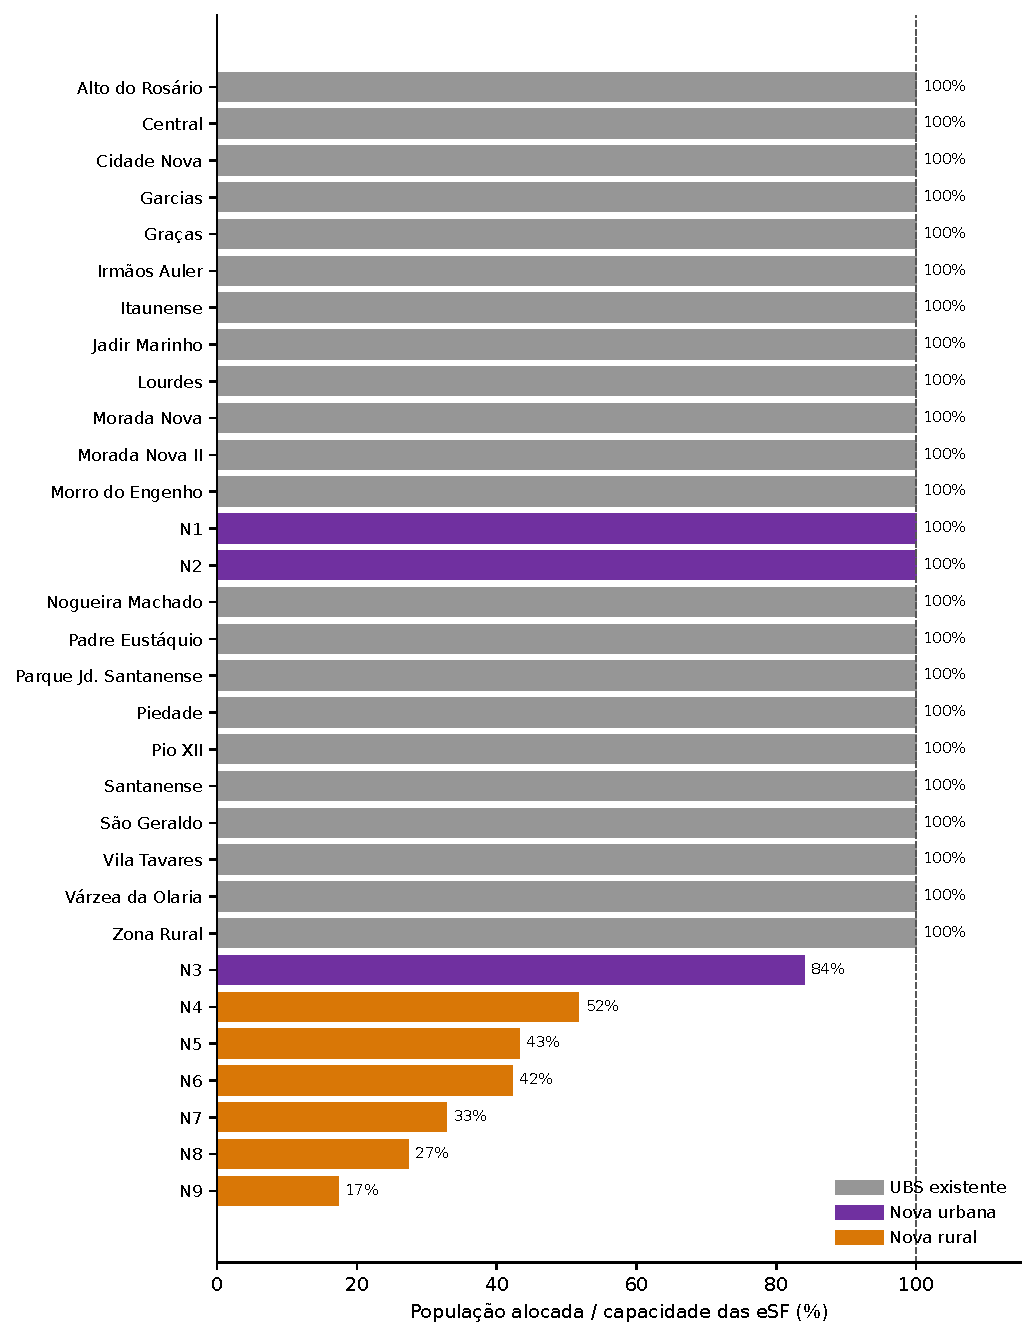
\includegraphics[width=.96\linewidth,height=.82\textheight,keepaspectratio]{figuras/ocupacao_equipes.pdf}
\caption{Ocupação das equipes fixas nas 31 UBS do plano, ordenada do maior para o menor percentual}\label{fig:utilizacao}
\fonte{Resultados do modelo de localização e dimensionamento.}
\nota{Ocupação = população alocada / (3.000 $\times$ eSF). As cores distinguem UBS existentes, novas urbanas e
novas rurais. N1 a N9 seguem a Tabela~\ref{tab:unidades}. As equipes móveis não entram no cálculo.}
\end{figure}

\begin{table}[htbp]\centering
\caption{Base do complemento móvel}\label{tab:movel}
\begin{tabular}{lrrr}\toprule UBS-base & Equipes & ACS & População atendida\\\midrule
UBS Alto do Rosário & 2 & 4 & 2.385,24\\
\bottomrule\end{tabular}
\fonte{Resultados do modelo do complemento móvel.}
\nota{Soluções com o mesmo número mínimo de equipes podem ter bases alternativas.}
\end{table}

\section{Funcionamento e investimento}

A Tabela~\ref{tab:custos} resume os custos estimados. O funcionamento da rede proposta custa
R\$ 3,00 milhões por mês, dos quais cerca de dois terços correspondem às 22 UBS existentes. A construção
das nove UBS soma R\$ 22,8 milhões, com R\$ 11,9 milhões nas seis rurais. A Tabela~\ref{tab:orcamento}
compara esses valores com a dotação de 2026. O funcionamento anual equivale a 70,7\% da dotação, contra
47,6\% da rede atual. A construção, por ser um investimento único, não entra nesses percentuais.

\begin{table}[htbp]\centering
\caption{Custos estimados da rede proposta}\label{tab:custos}
\begin{tabular}{lr}\toprule Componente & Valor (R\$)\\\midrule
UBS existentes (22), por mês & 2.024.060,25\\
UBS novas (9), por mês & 889.782,89\\
Pessoal das equipes móveis, por mês & 83.226,00\\
Funcionamento total, por mês & 2.997.069,14\\
Funcionamento total, por ano & 35.964.829,67\\
Construção das novas UBS (uma vez) & 22.848.000,00\\
\bottomrule\end{tabular}
\fonte{Resultados do modelo, com custos de referência descritos na Seção~\ref{sec:modeloaps} e \citet{novopac2025}.}
\nota{Veículos e combustível das equipes móveis, terrenos e equipamentos não foram precificados.}
\end{table}

\begin{table}[htbp]\centering
\caption{Custos estimados em relação à dotação atualizada da Atenção Básica de 2026}\label{tab:orcamento}
\begin{tabular}{lrr}\toprule Item & Valor anual (R\$) & \% da dotação\\\midrule
Dotação atualizada da Atenção Básica & 50.894.556,87 & 100,0\\
Rede atual, pessoal estimado e custos fixos & 24.232.528,33 & 47,6\\
Rede proposta, funcionamento & 35.964.829,67 & 70,7\\
\bottomrule\end{tabular}
\fonte{RREO, Anexo 02, quarto bimestre de 2026 \citep{tesouro2026}, e resultados do modelo.}
\nota{A dotação não é saldo livre, pois outras despesas da atenção primária não modeladas também a consomem.}
\end{table}

\section{Encaminhamentos especializados}\label{sec:encaminhamentos}

A Tabela~\ref{tab:ambulatorial} mostra os procedimentos alocados nos seis cenários, que combinam as duas
classificações com os três valores de $r$. A média complexidade é praticamente toda atendida em todos
eles. Na alta complexidade, a classificação única aloca 11.829 dos 15.863 procedimentos projetados, ou
74,6\%. A classificação de dois níveis eleva esse valor para 12.746, ou 80,3\%, e reduz a distância média
em cerca de 5\%. O volume de alta complexidade atendido não muda com $r$, e a média
complexidade só cai um pouco na classificação única com $r=75\%$.

\begin{table}[htbp]\centering
\caption{Procedimentos ambulatoriais alocados por cenário (procedimentos/ano)}\label{tab:ambulatorial}
\setlength{\tabcolsep}{5pt}
\begin{tabular}{llrrrr}\toprule
Classificação & Via sec. (\%) & Nível 2 & Nível 3 & Nível 3 atendido (\%) & Distância (km)\\\midrule
Única & 25 & 192.205,1 & 11.829,0 & 74,6 & 3,89\\
Única & 50 & 192.205,1 & 11.829,0 & 74,6 & 3,95\\
Única & 75 & 192.136,6 & 11.829,0 & 74,6 & 4,01\\
Dois níveis & 25 & 192.205,1 & 12.746,0 & 80,3 & 3,70\\
Dois níveis & 50 & 192.205,1 & 12.746,0 & 80,3 & 3,75\\
Dois níveis & 75 & 192.205,1 & 12.746,0 & 80,3 & 3,81\\
\bottomrule\end{tabular}
\fonte{Resultados do modelo de encaminhamento hierárquico.}
\nota{Distância média por percurso, em linha reta, ponderada pelos volumes atendidos. Como os volumes
alocados diferem entre cenários, as médias não se referem exatamente aos mesmos atendimentos.}
\end{table}

A Figura~\ref{fig:capacidades} explica a falta na alta complexidade. O hospital usa 38,1\% da sua
capacidade ambulatorial total, mas atinge 100\% do limite específico de alta complexidade, que não pode
ser ampliado com a capacidade que sobra. Os demais estabelecimentos atendem a média complexidade e
ficam no limite, exceto o centro de especialidades, que usa 72\% da sua capacidade.

\begin{figure}[htbp]\centering
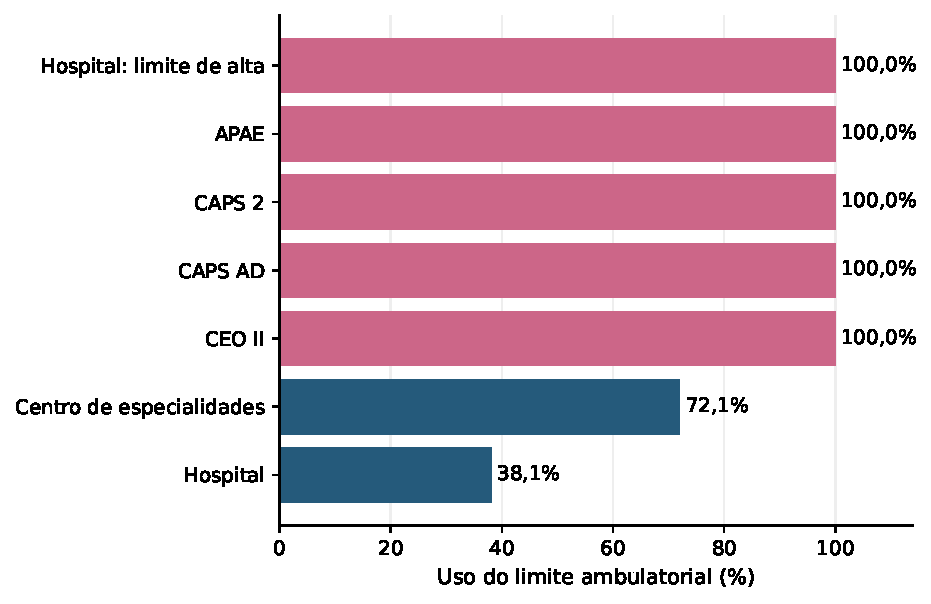
\includegraphics[width=.95\linewidth]{figuras/capacidades.pdf}
\caption{Uso dos limites ambulatoriais na classificação única, com 50\% via secundária, incluindo o limite
de alta complexidade do hospital}\label{fig:capacidades}
\fonte{Resultados do modelo de encaminhamento hierárquico.}
\end{figure}

As internações eletivas projetadas somam 1.072,5 de média e 352,5 de alta complexidade por ano e
exigiriam cerca de 6.676 dias-leito. No cenário conservador de leitos, nenhuma é alocada. No cenário
favorável, com 6.136 dias-leito, a classificação de dois níveis aloca 92,6\% das internações, enquanto a
classificação única aloca de 6\% a 19\% (Tabela~\ref{tab:leitos_otimista}). A diferença ocorre porque, na
classificação única, o hospital é apenas terciário e não recebe internações de média complexidade.

\begin{table}[htbp]\centering
\caption{Internações eletivas alocadas no cenário de disponibilidade hospitalar mais favorável}\label{tab:leitos_otimista}
\begin{tabular}{llrrr}\toprule Classificação & Via sec. (\%) & Média (\%) & Alta (\%) & Total (\%)\\\midrule
Única & 25 & 0,0 & 75,0 & 18,6\\
Única & 50 & 0,0 & 50,0 & 12,4\\
Única & 75 & 0,0 & 25,0 & 6,2\\
Dois níveis & 25 & 90,2 & 100,0 & 92,6\\
Dois níveis & 50 & 90,2 & 100,0 & 92,6\\
Dois níveis & 75 & 90,2 & 100,0 & 92,6\\
\bottomrule\end{tabular}
\fonte{Resultados do modelo de encaminhamento hierárquico com 6.136,35 dias-leito gerais.}
\nota{Percentual das internações/ano projetadas. O limite favorável é um extremo de sensibilidade, e não
capacidade residual observada. No cenário conservador, nenhuma internação é alocada.}
\end{table}

\section{Acessibilidade por zona}

A Tabela~\ref{tab:acessibilidade} mostra o índice de acessibilidade médio por zona, em valor absoluto e
relativo à média de cada rede. Na rede atual, o índice rural é 0,19 vez a média municipal com $\beta=1$ e
cai para 0,02 com $\beta=2$, que penaliza mais as distâncias longas. Na rede proposta, o índice rural
passa a superar a média, chegando a 1,10 com $\beta=1$, por causa das novas UBS rurais.

\begin{table}[htbp]\centering
\caption{Índice de acessibilidade médio por zona}\label{tab:acessibilidade}
\begin{tabular}{llrrr}\toprule Rede & Zona & $\beta$ & Índice absoluto & Índice relativo\\\midrule
Atual & Urbana & 1 & 0,689 & 1,04\\
Atual & Rural & 1 & 0,129 & 0,19\\
Atual & Urbana & 2 & 0,695 & 1,05\\
Atual & Rural & 2 & 0,013 & 0,02\\
Proposta & Urbana & 1 & 1,119 & 0,99\\
Proposta & Rural & 1 & 1,243 & 1,10\\
Proposta & Urbana & 2 & 1,006 & 0,89\\
Proposta & Rural & 2 & 3,583 & 3,19\\
\bottomrule\end{tabular}
\fonte{Resultados do diagnóstico de acessibilidade.}
\nota{A média municipal do índice absoluto é 0,663 na rede atual e 1,125 na proposta. O índice usa apenas as
eSF fixas e não é um percentual.}
\end{table}

\section{Sensibilidade}

A Tabela~\ref{tab:sensibilidade} altera um parâmetro de cada vez em relação ao cenário principal. A
curva de cobertura e custo, na Figura~\ref{fig:curva}, impõe metas mínimas de cobertura com capacidade, sem a folga de
2\%, e por isso o seu ponto de cobertura máxima custa um pouco menos que o cenário principal. O
custo inclui as equipes móveis necessárias para completar a cobertura. Com a meta de 93,4\%, são cinco
equipes móveis, o que torna esse ponto mais caro que o de 95\%. Metas acima de 97,7\% são inviáveis só
com UBS fixas.

A Figura~\ref{fig:investimento_cobertura} mostra, para os mesmos cenários, apenas o investimento em
construção. Cada ponto é um plano reotimizado para uma meta de cobertura, e o salto entre pontos mostra
quanto custa ampliar a meta. Para 93,4\% bastam três UBS urbanas. Cada meta acima disso exige
também unidades rurais, de uma em 95\% a seis em 97,7\%, e o investimento sobe até os R\$ 22,85 milhões
do cenário principal.

Um raio rural de 5 km reduz o número de UBS novas e eleva a cobertura rural de 53,5\% para 82,1\%, com
3 km na zona urbana, ou para 90,4\%, com 5 km nas duas zonas (Figura~\ref{fig:raios_cobertura}). Sem
mínimo de população rural, o plano abre 14 UBS, e com mínimo de 1.000 habitantes, apenas quatro. Com 5\%
e 10\% mais habitantes que em 2026, são necessárias 10 e 13 UBS novas. A folga de 5\% produz a mesma
solução do cenário principal.

\begin{table}[htbp]\centering\small
\caption{Sensibilidade do plano da atenção primária}\label{tab:sensibilidade}
\begin{tabular}{p{.36\linewidth}rrrrr}
\toprule Cenário & \shortstack{Novas\\UBS} & \shortstack{Cob.\\(\%)} & \shortstack{Equipes\\móveis} & \shortstack{Operação\\(mil R\$/mês)} & \shortstack{Construção\\(mi R\$)}\\\midrule
Principal (3 km, mínimo rural 500, folga 2\%) & 9 & 97,71 & 2 & 2.997,07 & 22,85\\
\midrule
\multicolumn{6}{l}{\textit{Curva de cobertura e custo (folga nula)}}\\
Cobertura mínima de 93,4\% & 3 & 93,40 & 5 & 2.888,87 & 12,92\\
Cobertura mínima de 95,0\% & 4 & 95,00 & 4 & 2.862,26 & 13,46\\
Cobertura mínima de 96,0\% & 5 & 96,00 & 4 & 2.863,21 & 14,90\\
Cobertura mínima de 97,0\% & 7 & 97,00 & 3 & 2.920,77 & 18,87\\
Cobertura máxima & 9 & 97,71 & 2 & 2.978,34 & 22,85\\
\midrule
\multicolumn{6}{l}{\textit{Raio de cobertura (urbano/rural)}}\\
2/2 km & 9 & 95,72 & 4 & 3.006,43 & 20,87\\
3/5 km & 8 & 99,03 & 1 & 2.912,89 & 20,86\\
5/5 km & 7 & 99,56 & 1 & 2.846,91 & 19,11\\
\midrule
\multicolumn{6}{l}{\textit{Mínimo de abertura rural}}\\
Sem mínimo & 14 & 99,86 & 1 & 3.191,69 & 32,79\\
1.000 habitantes & 4 & 94,81 & 4 & 2.866,94 & 13,46\\
\midrule
\multicolumn{6}{l}{\textit{Outros parâmetros}}\\
Folga operacional de 5\% & 9 & 97,71 & 2 & 2.997,07 & 22,85\\
População 5\% maior & 10 & 98,19 & 2 & 3.099,98 & 25,84\\
População 10\% maior & 13 & 99,07 & 1 & 3.279,18 & 32,12\\
\bottomrule\end{tabular}
\fonte{Resultados das análises de sensibilidade.}
\nota{Cob. é a cobertura com capacidade das UBS fixas, medida no raio de cada cenário, e por isso cenários
com raios diferentes não são diretamente comparáveis. A operação inclui as UBS e o pessoal das equipes
móveis. Metas de 98\%, 99\% e 99,5\% são inviáveis só com UBS fixas no raio de 3 km.}
\end{table}

\begin{figure}[htbp]\centering
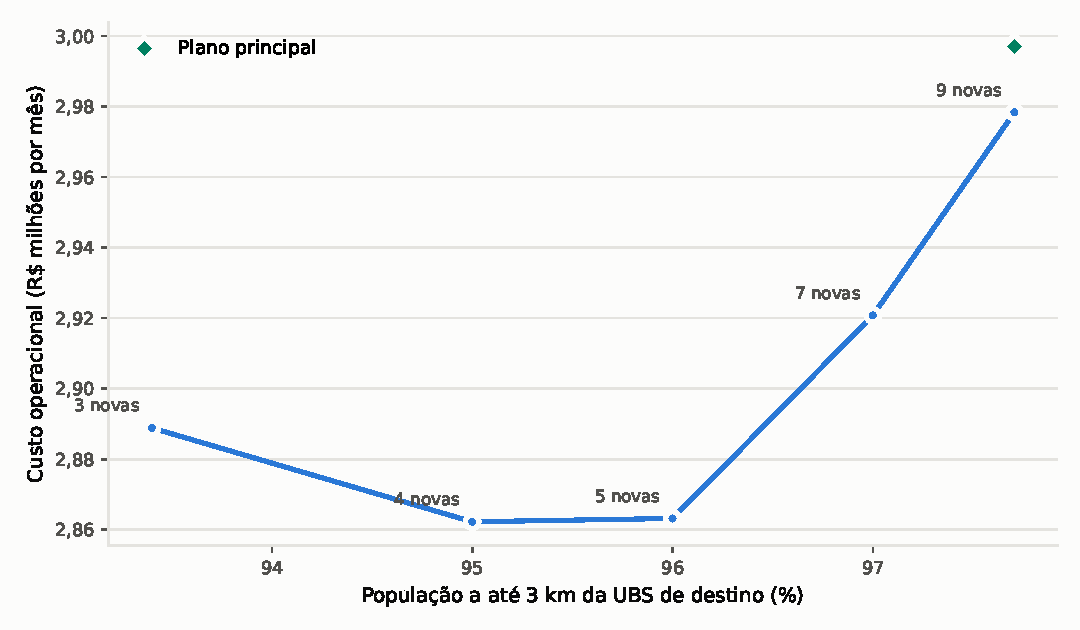
\includegraphics[width=.98\linewidth]{figuras/curva_cobertura_custo.pdf}
\caption{Custo operacional nos cenários de meta de cobertura com capacidade}\label{fig:curva}
\fonte{Resultados das análises de sensibilidade.}
\end{figure}

\begin{figure}[htbp]\centering
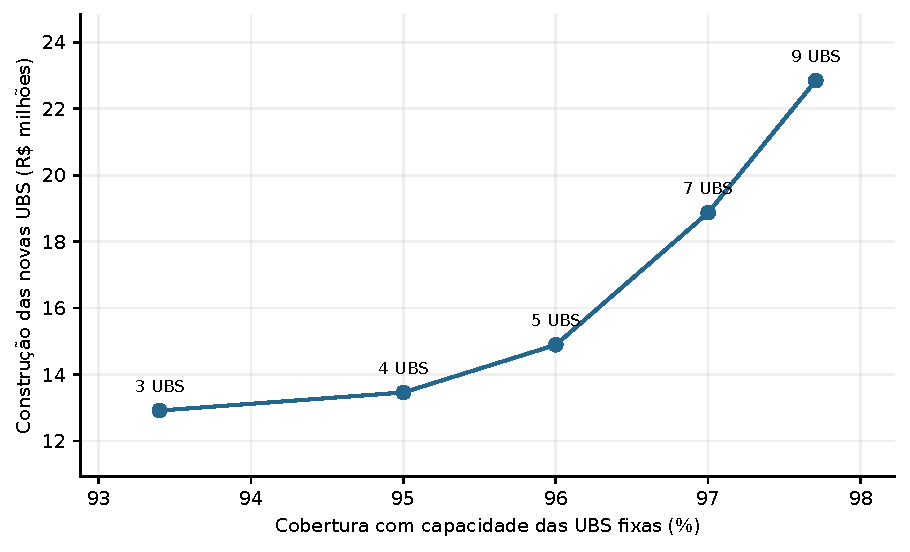
\includegraphics[width=.92\linewidth]{figuras/investimento_cobertura.pdf}
\caption{Investimento em construção nos cenários de meta de cobertura}\label{fig:investimento_cobertura}
\fonte{Resultados da análise de sensibilidade, com custos por porte do Novo PAC Saúde \citep{novopac2025}.}
\nota{Raio de 3 km e folga operacional nula. O eixo vertical inclui apenas a construção das UBS. Os rótulos
indicam quantas novas UBS cada plano abre.}
\end{figure}


\begin{figure}[htbp]\centering
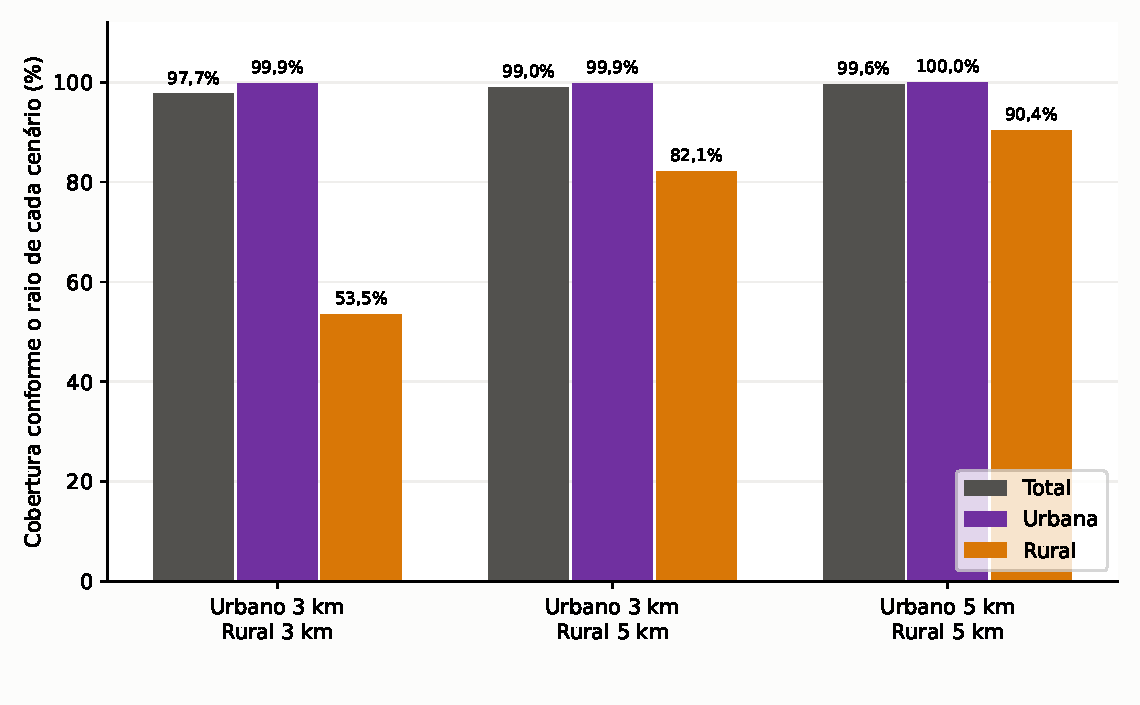
\includegraphics[width=.9\linewidth]{figuras/extra_raios_02_cobertura.pdf}
\caption{Cobertura total, urbana e rural nos cenários de raio}\label{fig:raios_cobertura}
\fonte{Resultados das análises de sensibilidade.}
\end{figure}
